\documentclass[10pt,a4paper,oneside]{article}
\usepackage[latin1]{inputenc}
\usepackage{amsmath}
\usepackage{amsfonts}
\usepackage{amssymb}
\usepackage{graphicx}
\usepackage{booktabs}
\usepackage{tabularx}
\graphicspath{{figures/}}
\newcommand\nlgn{$ \Theta(n\lg n) $}
\newcommand\nn{$ \Theta(n^2) $}
\def\c{$ \Theta(1) $}
\newcommand\n{$ \Theta(n) $}
\newcommand\lgn{$ \Theta(\lg n) $}
\author{Simon Virenfeldt}
\title{Algorithms and Data Structures - Reference}
\date{2017\\September - January}
\begin{document}
    \maketitle
    \section{Standard notation and common functions}
    \textit{CLRS section 3.2 p. 53}
\subsection{Monotonicity}
A function $ f(n) $ is
\begin{description}
    \item[monotonically increasing] if $ m \leq n $ implies $ f(m) \leq f(n) $.
    \item[monotonically decreasing] if $ m \leq n $ implies $ f(m) \geq f(n) $.
    \item[strictly increasing] if $ m < n $ implies $ f(m) < f(n) $.
    \item[strictly decreasing] if $ m < n $ implies $ f(m) > f(n) $.
\end{description}

\subsection{Exponentials}
For all real $ a > 0$, $ b > 0 $, $ m $, and $ n $, we have the following identities:\\
\begin{align*}
a^0 &= 1\\
a^1 &= a\\
a^{-1} &= \frac{1}{a}\\
\left( a^m\right) ^n &= a^{nm}\\
\left( a^m\right) ^n &= \left( a^n\right) ^m\\
a^ma^n &= a^{n+m}\\
0^0&=1\\
a^mb^m&=(ab)^m\\
a^\frac{m}{n} &= \left( \sqrt[n]{a}\right) ^m\\
a^{-m}&=\dfrac{1}{a^m}\\
a^{m-n}&=\dfrac{a^m}{a^n}
\end{align*}
\subsection{Logarithms}
\emph{Logarithm functions apply only to the next term in the formula}, so that $ \lg n + k $ will mean $ \left( \lg n\right) +k $ and not $ \lg(n+k) $.
CLRS uses the following notations:
\begin{align*}
\lg n &= \log_2 n &\text{(binary logarithm)}\\
\ln n &= \log_e n &\text{(natural logarithm)}\\
\lg^kn &= (\lg n)^k &\text{(exponentiation)}\\
\lg\lg n &= \lg (\lg n) &\text{(composition)}
\end{align*}
For all real $ a > 0 $, $ b > 0 $, $ c > 0 $, and $ n $,
\begin{align*}
a &= b^{\log_ba}\\
\log_c(ab) &= \log_ca+\log_cb\\
\log_ba^n &= n\log_ba\\
\log_ba &= \dfrac{\log_ca}{\log_cb}\\
\log_b\left( \frac{1}{a}\right) &= -\log_ba\\
\log_ba &= \dfrac{1}{\log_ab}\\
a^{\log_bc}&=c^{\log_ba}\\
\log_b 1 &= 0\\
\log_bb &= 1\\
\log_b\left( \frac{a}{c}\right) &= \log_b a - \log_b c
\end{align*}
where, in each equation above, logarithm bases are not 1.\\

There is a simple series expansion for $ \ln (1+x) $ when $ |x| < 1 $:
$$ \ln(1+x) = x - \dfrac{x^2}{2} + \dfrac{x^3}{3} - \dfrac{x^4}{4} + \dfrac{x^5}{5} - \cdots $$

We also have the following inequalities for $ x > -1 $:
$$ \dfrac{x}{1+x} \leq \ln(1+x) \leq x $$
where equality holds only for $ x = 0 $.
    \section{The master method}
    \textit{CLRS section 4.5 p. 93}
Let $ a \ge 1 $ and $ b > 1 $ be constants, let $ f(n) $ be a function, and let $ T(n) $ be defined on the nonnegative integers by the recurrence
$$ T(n) = aT\left( \frac{n}{b}\right) + f(n), $$
where we interpret $ \frac{n}{b} $ to mean either $ \lfloor \frac{n}{b}\rfloor $ or $ \lceil\frac{n}{b} \rceil$.
Then $ T(n) $ has the following asymptotic bounds:
\begin{enumerate}
    \item If $ f(n)=O\left( n^{\log_ba-\epsilon} \right) $ for some constant $ \epsilon > 0 $, then $ T(n)=\Theta\left( n^{\log_ba}\right)$.
    \item If $ f(n)=\Theta\left( n^{\log_ba}\right) $, then $ T(n)=\Theta\left( n^{log_ba}\lg n\right)  $.
    \item If $ f(n)=\Omega\left( n^{\log_ba+\epsilon}\right)  $ for some constant $ \epsilon > 0 $, and if $ af\left( \frac{n}{b}\right) \leq cf(n) $ for some constant $  c < 1 $ and all sufficiently large $ n $, then $ T(n)=\Theta(f(n)) $.
\end{enumerate}
\subsection{Using the master method}
\begin{enumerate}
    \item Determine if the recurrence is on the form $ T(n) = aT\left( \frac{n}{b}\right) + f(n) $.
    \item Extract $ a $, $ b $, and $ f(n) $ from the recurrence.
    \item Determine $ n^{\log_b a} $.
    \item Compare $ f(n) $ and $ n^{\log_b a} $ asymptotically.
    \begin{enumerate}
        \item If $ f(n) $ increases polynomially slower then $ T(n)=\Theta\left( n^{\log_ba}\right)$.
        \item If $ f(n) $ increases similarly then $ T(n)=\Theta\left( n^{log_ba}\lg n\right)  $.
        \item If $ f(n) $ increases polynomially faster and if $ af\left( \frac{n}{b}\right) \leq cf(n) $ for some constant $  c < 1 $ and all sufficiently large $ n $, then $ T(n)=\Theta(f(n)) $.
    \end{enumerate}
\end{enumerate}
    \section{Summations}
    \textit{CLRS appendix A page 1145}

\subsection{Linearitet}
For any real number $ c $ and any finite sequences $ a_1,a_2,\ldots,a_n $ and $ b_1,b_2,\ldots,b_n $,
$$ \sum_{k=1}^{n}\left( ca_k+b_k\right) = c \sum_{k=1}^{n}a_k + \sum_{k=1}^{n}b_k. $$

\subsection{Arithmetic series}
The summation
$$ \sum_{k=1}^{n}k = 1+2+\cdots+n $$
is an \textbf{\textit{arithmetic series}} and has the value
\begin{align*}
\sum_{k=1}^{n}k &= \dfrac{1}{2}n(n+1)\\
&= \Theta\left( n^2\right) .
\end{align*}

\subsection{Sums of squares and cubes}'
We have the following summations of squares and qubes:
\begin{align*}
\sum_{k=0}^{n}k^2&=\dfrac{n(n+1)(2n+1)}{6}\\
\sum_{k=0}^{n}k^3&=\dfrac{n^2(n+1)^2}{4}.
\end{align*}

\subsection{Geometric series}
For real $ x \neq 1 $, the summation
$$ \sum_{k=0}^{n}x^k = 1+x+x^2+\cdots+x^n $$
is a \textit{\textbf{geometric}} or \textbf{\textit{exponential series}} and has the value
$$ \sum_{k=0}^{n}x^k = \dfrac{x^{n+1}-1}{x-1} $$

    \section{Asymptotic notation}
    \subsection{Comparing functions}
\textit{CLRS section 3.1 page 51}
For the following, assume that $ f(n) $ and $ g(n) $ are asymptotically positive.
\subsubsection{Transitivity}
\begin{alignat*}{11}
	&f(n) &&= \Theta(g(n)) &\quad\text{and}\quad g(n) &&= \Theta(h(n)) &\quad\text{imply}\quad f(n) &&= \Theta(h(n))\\
	&f(n) &&= O(g(n)) 	&\quad\text{and}\quad g(n) &&= O(h(n)) &\quad\text{imply}\quad f(n) &&= O(h(n))\\
	&f(n) &&= \Omega(g(n)) 	&\quad\text{and}\quad g(n) &&= \Omega(h(n)) &\quad\text{imply}\quad f(n) &&= \Omega(h(n))\\
	&f(n) &&= o(g(n)) 	&\quad\text{and}\quad g(n) &&= o(h(n)) &\quad\text{imply}\quad f(n) &&= o(h(n))\\
	&f(n) &&= \omega(g(n)) 	&\quad\text{and}\quad g(n) &&= \omega(h(n)) &\quad\text{imply}\quad f(n) &&= \omega(h(n))
\end{alignat*}

\subsubsection{Reflexivity}
\begin{align*}
	f(n) &= \Theta(f(n))\\
	f(n) &= O(f(n))\\
	f(n) &= \Omega(f(n))
\end{align*}

\subsubsection{Symmetry}
$$ f(n)=\Theta(g(n)) \text{ if and only if } g(n)=\Theta(f(n)) $$ 

\subsubsection{Transpose symmetry}
\begin{alignat*}{3}
	&f(n) &&= O(g(n)) \quad\text{if and only if}\quad  g(n) &&= \Omega(f(n))\\
	&f(n) &&= o(g(n)) \quad\text{if and only if}\quad  g(n) &&= \omega(f(n))
\end{alignat*}

\subsection{The engineering way}
Ignore its leading constants: $ T(n)=1000n^5 = \Theta(n^5) $.\\
Drop its low order terms: $ T(n)=n^5+n^3+\lg n = \Theta(n^5) $\\
\textbf{Identifying lower order terms}
\[
\begin{array}{ccccccc}
	\text{Constant} &<& \text{Poly-logarithm} &<& \text{Polynomial} &<& \text{Exponential}\\
	c &<& \lg^kn &<& n^a &<& b^n
\end{array}
\]
    \section{Loop invariants}
    To show that a loop invariant holds 3 things must be true:\textit{(CLRS page 19)}
\begin{description}
	\item[Initialization] It is true prior to the first iteration of the loop.
	\item[Maintenance] If it is true before an iteration of the loop, it remains true before the next iteration.
	\item[Termination] When the loop terminates, the invariant gives us a useful property that helps show that the algorithm is correct.
\end{description}
    \section{Sorting algorithms}
    \begin{tabularx}{\linewidth}{lXXX}
	\toprule
	               & \textbf{Worst case run time} & \textbf{Average case run time} & \textbf{In place or not?}      \\ \midrule
	Merge Sort     & \nlgn                        & \nlgn                          & No. $ \Theta(n) $.             \\
	Insertion Sort & \nn                          & \nn                            & Yes. $ \Theta(1) $ additional. \\
	Bubble Sort    & \nn                          & \nn                            & Yes.                           \\
	Selection Sort & \nn                          & \nn                            & Yes.                           \\
	Quick Sort     & \nn                          & \nlgn                          & Yes.                           \\
	Heap Sort      & \nlgn                        & \nlgn                          & Yes.                           \\ \bottomrule
\end{tabularx}

\subsection{Behavior of sorting algorithms}

\begin{description}
	\item[Merge sort] (CLRS p.29-34) Divide-and-conquer. Recursively split list into two sublists of equal size, then merge the sorted sublists by comparing the front elements and taking the smallest until both lists are empty. 
	\item[Insertion sort] (CLRS p.17-18) Runs through the list, and places the $j$th element in the correct place out of the sublist $A[1..j-1]$, the already sorted elements. 
	\item[Bubble sort] (CLRS p.40, Problem 2-2) Sorts by repeatedly looping through the list, swapping out of order elements. The bigger elements slowly "bubble" upwards. 
	\item[Selection sort] (CLRS p.29, Exercise 2.2-2) Runs through the list and takes the smallest unsorted element and places it in front of the array. 
	\item[Quick sort] (CLRS Chapter 7, p.170 onwards) Takes some pivot element $x$ from a place in the list, and places all elements smaller than $x$ to the left of $x$, and all elements bigger to the right. Then it recursively quicksorts the sublists of elements smaller than $x$ and bigger than $x$.
	\item[Heap sort] (CLRS Chapter 6, p.151 onwards) Constructs a max heap out of the array. Then it repeatedly exchanges the maximum element with the last element in the heap, then heapifies again. 
	\subitem \textsc{Max-Heapify}(i): Assuming that the trees at \textsc{Left}(i) and \textsc{Right}(i) are heaps, make the tree rooted at $i$ a heap. 
\end{description}
    \section{Abstract data types}
    \subsection{Dynamic set}
A dynamic set is a grouping of values.
A dynamic set implements some or all of the following operations specified on \textbf{page 230}.\\
\begin{tabularx}{\linewidth}{Xlp{1.2cm}lll}
	\toprule
	                           & \textbf{Max} & \textbf{Extract-Max} & \textbf{Insert} & \textbf{Delete} & \textbf{Search} \\ \midrule
	Heap                       & \c               & \lgn                 & \lgn            & \lgn            & \n              \\
	Singly Linked List         & \n               & \n                   & \c              & \n              & \n              \\
	Ordered singly linked list & \c               & \c                   & \n              & \n              & \n              \\
	Doubly linked list         & \n               & \n                   & \c              & \c              & \n              \\
	Ordered doubly linked list & \c               & \c                   & \n              & \c              & \n              \\
	Hash table                 & \n               & \n                   & \c              & \c              & \c              \\ \bottomrule
\end{tabularx}
\subsection{Stack}
\textit{CLRS section 10.1 page 232}\\
A stack is a container of objects. Objects are inserted and removed according to the last-in-first-out (LIFO) principle.
A stack has the following operations:
\begin{description}
	\item[Push($ S $, $ x $)] inserts an element $ x $ into the stack $ S $.
	\item[Pop($ S $)] deletes the element on top of the stack $ S $. 
	\item[Stack-Empty($ S $)] returns whether the stack is empty.
\end{description}

\subsection{Queue}
\textit{CLRS section 10.1 page 234}\\
A queue is a container of elements. Elements are inserted and removed according to the First-in-first-out (FIFO) principle.
A queue has the following operations:
\begin{description}
	\item[Enqueue($ Q $, $ x $)] inserts an element $ x $ into the queue $ Q $.
	\item[Dequeue($ Q $)] deletes the head element in the queue $ Q $, and returns is. 
\end{description}

\subsection{linked list}
\textit{Linked lists} and \textit{doubly linked lists} supports all og the operations on \textbf{page 230}.

\subsection{Priority Queue}
A priority queue (PQ) is a data structure for maintaining a set $ A $ of elements, each with an associated value called key.
A priority queue supports the following operations:
\begin{description}
	\item[Insert($ A $, $ x $)]  insert element $ x $ in set $ A (A=A\cup{x}) $.
	\item[Maximum($ A $)] returns the element of $ A $ with the largest key.
	\item[Extract-Max($ A $)] returns and removes the element of $ A $ with the
	largest key from $ A $.
\end{description}

\subsection{Dictionary}
Dictionaries store elements so that they can be located quickly using keys.
A dictionary supports the following operations:
\begin{description}
	\item[Search($ S $, $ k $)] an access operation that returns a pointer $ x $ to an element where $ x.key = k $.
	\item[Insert($ S $, $ x $)] a manipulation operation that adds element $ x $ to $ S $.
	\item[Delete($ S $, $ x $)] a manipulation operation that removes element $ x $ from $ S $.
\end{description}
    \section{Tree walks}
    \begin{figure}[h]
	\centering
	\begin{minipage}{0.3\textwidth}
		\centering
		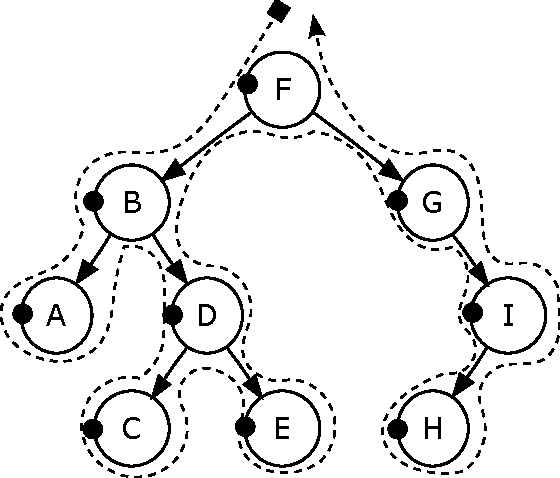
\includegraphics[width=\textwidth]{Sorted_binary_tree_preorder}
		\caption{Pre-order tree walk}
	\end{minipage}
	\hfill
	\begin{minipage}{0.3\textwidth}
		\centering
		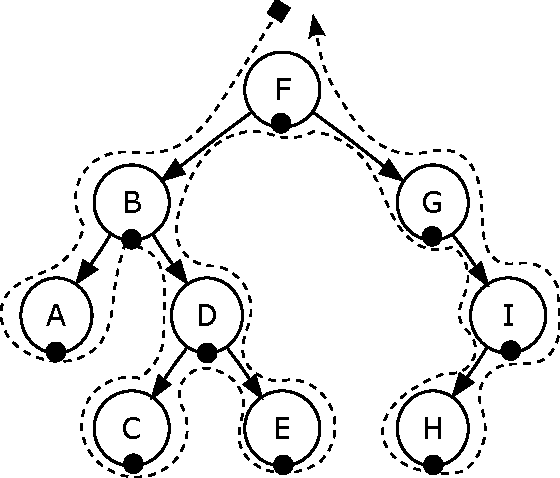
\includegraphics[width=\textwidth]{Sorted_binary_tree_inorder}
		\caption{In-order tree walk}
	\end{minipage}
	\hfill
	\begin{minipage}{0.3\textwidth}
		\centering
		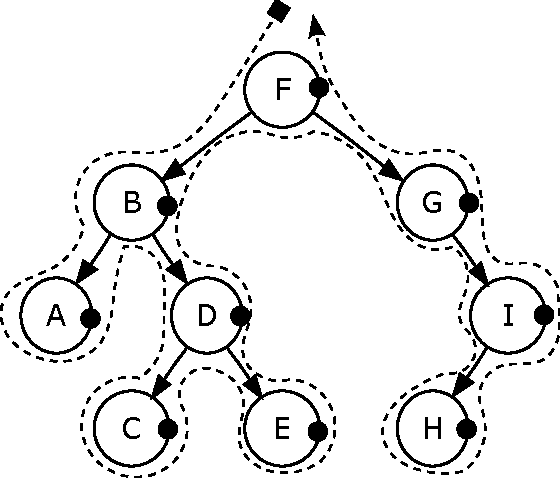
\includegraphics[width=\textwidth]{Sorted_binary_tree_postorder}
		\caption{Post-order tree walk}
	\end{minipage}	
\end{figure}
    \section{Fractions identities}
    \subsection{Negative fractions}
\begin{align*}
-\frac{a}{b}&=\frac{-a}{b}=\frac{a}{-b}\\
\frac{-a}{-b}&=\frac{a}{b}\\
-\frac{a}{b}&\neq \frac{-a}{-b}
\end{align*}
\subsection{Cancellation}
\begin{align*}
\frac{a}{a}&=1\\
\frac{ab}{ac}&=\frac{b}{c}\\
a*\frac{b}{a}&=b
\end{align*}
\subsection{Addition}
\begin{align*}
\frac{a}{b}+\frac{c}{b}&=\frac{a+c}{b}\\
a+\frac{b}{c}=\frac{ac}{c}+\frac{b}{c}&=\frac{ac+b}{c}\\
\frac{a}{b}+\frac{c}{d}=\frac{ad}{bd}+\frac{bc}{bd}&=\frac{ad+bc}{bd}
\end{align*}
\subsection{Subtraction}
\begin{align*}
\frac{a}{b}-\frac{c}{b}&=\frac{a-c}{b}\\
a-\frac{b}{c}=\frac{ac}{c}-\frac{b}{c}&=\frac{ac-b}{c}\\
\frac{a}{b}-c=\frac{a}{b}-\frac{bc}{b}&=\frac{a-bc}{b}\\
\frac{a}{b}-\frac{c}{d}=\frac{ad}{bd}-\frac{bc}{bd}&=\frac{ad-bc}{bd}
\end{align*}
\subsection{Multiplication}
\begin{align*}
\frac{a}{b}*\frac{c}{d}&=\frac{ac}{bd}\\
a*\frac{b}{c}=\frac{a}{1}*\frac{b}{c}&=\frac{ab}{c}\\
\frac{a}{b}*c=\frac{a}{b}*\frac{c}{1}&=\frac{ac}{b}
\end{align*}
\subsection{Division}
\begin{align*}
\dfrac{\dfrac{a}{b}}{\dfrac{c}{d}}=\dfrac{a}{b}*\dfrac{d}{c}&=\dfrac{ad}{bc}\\
\dfrac{\frac{a}{b}}{c}=\dfrac{\frac{a}{b}}{\frac{c}{1}}=\frac{a}{b}*\frac{1}{c}&=\frac{a}{bc}\\
\dfrac{a}{\frac{b}{c}}=\dfrac{\frac{a}{1}}{\frac{b}{c}}=\frac{a}{1}*\frac{c}{b}&=\frac{ac}{b}
\end{align*}
\subsection{OBS!}
\begin{align*}
\frac{a}{c}*\frac{b}{c}&\neq\frac{ab}{c}\\
2\frac{1}{3}&=2+\frac{1}{3}\\
2\frac{1}{3}&\neq 2*\frac{1}{3}
\end{align*}
    \section{Root identities}
    \subsection{Definitions}
\begin{align*}
b&=\sqrt{a} : b \geq 0 \wedge b^2=a \\
\sqrt{a^2}&= \vert a \vert \\
\text{If } a&\geq \text{ then } \sqrt{a^2}=a
\end{align*}
\subsection{Distributing}
$(a\geq 0 \wedge b\geq 0)$
\begin{align*}
\sqrt{ab}&=\sqrt{a}\sqrt{b} \\
\sqrt{\frac{a}{b}}&= \frac{\sqrt{a}}{\sqrt{b}}\qquad(b\neq 0) \\
\sqrt{a}\sqrt{a}&=a\\
\sqrt{a^n}&=\left( \sqrt{a} \right) ^n \vee a^{\frac{n}{2}}
\end{align*}
\subsection{Rationalizing the Denominator}
$(a>0 \wedge b>0 \wedge c>0)$
\begin{align*}
\frac{a}{\sqrt{b}}=\frac{a}{\sqrt{b}}\cdot\frac{\sqrt{b}}{\sqrt{b}}&=\frac{a\sqrt{b}}{b} 
&
\frac{4}{\sqrt{2}}=\frac{4}{\sqrt{2}}\cdot\frac{\sqrt{2}}{\sqrt{2}}&=\frac{4\sqrt{2}}{2}=2\sqrt{2} \\ \\
\frac{a}{b+\sqrt{c}}=\frac{a}{b+\sqrt{c}}\cdot \frac{b-\sqrt{c}}{b-\sqrt{c}}&=\frac{ab-a\sqrt{c}}{b^2-c}
&
\frac{6}{3+\sqrt{7}}=\frac{6}{3+\sqrt{7}}\cdot\frac{3-\sqrt{7}}{3-\sqrt{7}}&=\frac{18-6\sqrt{7}}{9-7} \\
& & = \frac{18-6\sqrt{7}}{9-7}=\frac{18-6\sqrt{7}}{2}&=9-3\sqrt{7} \\ \\
\frac{a}{b-\sqrt{c}}=\frac{a}{b-\sqrt{c}} \cdot \frac{b+\sqrt{c}}{b+\sqrt{c}} &= \frac{ab+a\sqrt{c}}{b^2-c}
&
\frac{5}{2-\sqrt{3}}=\frac{5}{2-\sqrt{3}}\cdot\frac{2+\sqrt{3}}{2+\sqrt{3}}&=\frac{10+5\sqrt{3}}{4-3} \\
& & =\frac{10+5\sqrt{3}}{1}&=10+5\sqrt{3} \\ \\
\frac{a}{\sqrt{b}+\sqrt{c}}=\frac{a}{\sqrt{b}+\sqrt{c}}\cdot \frac{\sqrt{b}-\sqrt{c}}{\sqrt{b}-\sqrt{c}}&=\frac{a\sqrt{b}-a\sqrt{c}}{b-c}
&
\frac{14}{\sqrt{13}+\sqrt{11}}=\frac{14}{\sqrt{13}+\sqrt{11}}\cdot \frac{\sqrt{13}-\sqrt{11}}{\sqrt{13}-\sqrt{11}}&=\frac{14\sqrt{13}-14\sqrt{11}}{13-11}\\
& & = \frac{14\sqrt{13}-14\sqrt{11}}{2}&=7\sqrt{13}-7\sqrt{11} \\ \\
\frac{a}{\sqrt{b}-\sqrt{c}}=\frac{a}{\sqrt{b}-\sqrt{c}}\cdot \frac{\sqrt{b}+\sqrt{c}}{\sqrt{b}+\sqrt{c}}&=\frac{a\sqrt{b}+a\sqrt{c}}{b-c}
&
\frac{12}{\sqrt{15}-\sqrt{7}}=\frac{12}{\sqrt{15}-\sqrt{7}} \cdot \frac{\sqrt{15}+\sqrt{7}}{\sqrt{15}+\sqrt{7}}&=\frac{12\sqrt{15}+12\sqrt{7}}{15-7}\\
& & = \frac{12\sqrt{15}+12\sqrt{7}}{8}&=\frac{3\sqrt{15}+2\sqrt{7}}{2}
\end{align*}
\subsection{OBS!}
\begin{align*}
\sqrt{a+b}&\neq \sqrt{a}+\sqrt{b}\\
\sqrt{a-b}&\neq \sqrt{a}-\sqrt{b}\\
\sqrt{a^2+b^2}&\neq a+b
\end{align*}

\end{document}